%\newpage


\appendix


\section{Further Examples}


\begin{example}[join on non-key columns]\em
\label{ex:nation}
Given an additional supplier relation, we now ask, for each supplier id (sid),
for the number of customers of the same nation.
\begin{verbatim}
SELECT   S.sid, SUM(1)
FROM     Customer C, Supplier S
WHERE    C.nation = S.nation
GROUP BY S.sid;
\end{verbatim}
The compiler produces the following triggers.
\begin{verbatim}
on insert into Customer (cid, nation) {
  (sid: Supplier.sid) q[sid] += qC[sid, nation];
  qS[nation] += 1
}
on insert into Supplier (sid, nation) {
  q[sid] += qS[nation];
  qC[sid, nation] += 1
}
\end{verbatim}
To understand that this pair
(quadruple, if the deletion triggers are taken into account) of
mutually dependent triggers indeed correctly maintains the query result in q,
verify that auxiliary map {\tt qS} maintains the query
\begin{verbatim}
SELECT nation, SUM(1) FROM Customer GROUP BY nation;
\end{verbatim}
and auxiliary map qC maintains query
\begin{verbatim}
SELECT   sid, nation, SUM(1) FROM Supplier
GROUP BY sid, nation;
\end{verbatim}
The statements updating {\tt q} assure that,
whenever a customer (resp., supplier) is inserted, the count of
matching suppliers (resp., customers) is added to {\tt q}.
\punto
\end{example}


\begin{example}[self-join with complex condition]\em
\label{ex:matchmaking}
In this final example, we consider the data\-base of a matchmaking Web site
that matches humans based on personal profiles. Persons are
represented by a relation Person(\underline{id}, prop), where
prop stands for possibly multiple property col\-umns. Let score$(\cdot, \cdot)$
be a function that maps a pair of property tuples to a compatibility score.
The following query computes, for each person in the database, the number of
matches with compatibility score $\ge 0.9$.
\begin{verbatim}
SELECT   P1.id, SUM(1)
FROM     Person P1, Person P2
WHERE    P1.id <> P2.id
AND      0.9 <= score(P1.prop, P2.prop)
GROUP BY P1.id;
\end{verbatim}

Our compilation approach turns this query into the following M3 program,
with map {\tt q[.]} representing the query result and auxiliary
maps {\tt q1[.,.]} and {\tt q2[.,.,.]}.
\begin{verbatim}
on insert into Person (id, prop) {
  q[id] += q1[id, prop];

  (id2: Person.id) q[id2] += q2[id2, id, prop];

  ((id1, prop1): Person)
  q1[id1, prop1] +=
    if id1<>id and 0.9<=score(prop1, prop) then 1
    else 0;

  ((id2, prop2): Person)
  q2[id, id2, prop2] +=
    if id<>id2 and 0.9<=score(prop, prop2) then 1
    else 0
}
\end{verbatim}
Note that whenever we read a value in such a map program, it has to be
the version of the value from before the start of the program. This is 
ensured in this program because we write q1 and q2 in entries 3 and 4 only
after we have read from q1 and q2 in the first two entries.
But note in particular that also the domains
(id2: Person.id), ((id1, prop1): Person), ((id2, prop2): Person)
are the old ones, before the insertion of the current tuple (id, prop).

The program again has the property that for
each map value to be written, only constantly much work has to be done,
and constantly many lookups have to be made.

This program is the conceptually most difficult so far, so let us look at it
in more detail. It is easy to see that entries 3 and 4 of the program
maintain q1 and q2 as the queries
\begin{verbatim}
q1[id, prop] =
SELECT SUM(1) FROM Person P2
WHERE id<>P2.id and 0.9<=score(prop, P2.prop) 

q2[id1, id, prop] =
SELECT SUM(1) FROM Person P1
WHERE P1.id<>id and 0.9<=score(P1.prop, prop)
AND   P1.id=id1 
\end{verbatim}

Now entry 1 of the program sets the q value for the new person, and
entry 2 updates the q values of the persons that were present previously.
For example, suppose score() is 1 on all inputs and assume that, currently,
there are three persons. Then q is two for each id. Now add a fourth person.
Then q1 is three for the new person and q2 is one for each of the old persons.
By default, q is 0 for the new person before the update.
%
\begin{center}
\begin{tabular}{c|c|c|c|c}
   & before    & \multicolumn{3}{c}{after insert} \\
id & q[id]     & q1[id,.] & q2[id,.,.] & q[id] \\
\hline
1  & 2         &          & 1          & 3 \\
2  & 2         &          & 1          & 3 \\
3  & 2         &          & 1          & 3 \\
4  & undef./0  & 3        &            & 3 \\
\end{tabular}
\end{center}
%
After execution of the on-insert trigger, q is three for each of the four
persons.
\punto
\end{example}


\subsection{Delta processing}


\begin{example}\em
Consider the query
\begin{verbatim}
SELECT SUM(r1.A * r2.B) FROM R r1, R r2
WHERE r1.B=r2.A;
\end{verbatim}
over relation $R$ of schema $(A,B)$
whose deltas on insertion/deletion of
$R$-tuples is
$\duv \AggSum(x*z, R(x,y) \land R(y,z))$ =
$\AggSum(x*z, \duv (R(x,y) \land R(y,z)))$
because $\duv (x*z) = 0$. Since
$\duv R(x,y) = (x=u \land y=v)$ and
$\duv R(y,z) = (y=u \land z=v)$,%
%
\begin{multline*}
\AggSum(x*z, \duv (R(x,y) \land R(y,z))) = \\
\AggSum(x*z, ((x=u \land y=v)^\pm \land R(y,z)) \\
\lor\;
 (R(x,y) \land (y=u \land z=v)^\pm) \\
\lor\;
 ((x=u \land y=v)^\pm \land (y=u \land z=v)^\pm)) =
\end{multline*}

\vspace{-6mm}

\begin{eqnarray*}
&\pm& \AggSum(x*z, x=u \land y=v \land R(y,z)) \\
&\pm& \AggSum(x*z, R(x,y) \land y=u \land z=v) \\
&+  & \AggSum(x*z, x=u \land y=v \land y=u \land z=v).
\end{eqnarray*}
Assuming no other bound variables than $u$ and $v$,
this simplifies to
$\pm \AggSum(u*z, R(v,z))
 \pm \AggSum(x*v, (R(x,u))
 +   (\mbox{if }(u=v) \mbox{ then }(u*v)\mbox{ else }0)$.

Now suppose $R$ currently stores $\{\!| (1,1), (1,1) |\!\}$
(i.e., two copies of tuple $(1,1)$; the query has value 4)
and we insert another copy of tuple $(1,1)$.
Then $\Delta_{+R(1,1)} = 2 + 2 + 1 = 5$, which is
correct: the new value of the query is 9. Now if we delete one of the tuples
$(1,1)$,
$\Delta_{-R(1,1)} = -3 -3 +1 = -5$, and we get back to query value 4. 
\punto
\end{example}


\nop{
Note that $u$ and $v$ are bound variables (to be treated like constants).
Thus, for instance,
$\AggSum(u, R(v, v))$ corresponds to SQL
select u from R where R.A=v and R.B=v,
where we assume that the schema of $R$ is $(A,B)$.
} % end nop


\subsection{Compilation}


\begin{example}\em
Consider a simplified TPC-H like schema with relations O(K, R)
and L(K, P). Orders O have an order key K and the current exchange rate R fixed for this order (for
foreign customers). Line items L have an {\em order} key
K and a price P. We compile the query
\begin{verbatim}
SELECT SUM(L.P * O.R) FROM O, L WHERE O.K = L.K
\end{verbatim}
which asks for the sum total of all LineItem prices weighted by the exchange
rates of their orders.

The corresponding calculus term is
\[
q[] = \AggSum(p*r, O(k, r) \land L(k, p)).
\]
There are no group-by columns, so we compile as Compile($q$, $\emptyset$, $t$).
We first compute the (insertion) delta for $O$,
\[
\Delta_{+O(k_{O}, r_{O})} q =
\AggSum(p*r, k=k_{O} \land r=r_{O} \land L(k, p))
\]
and simplify with bound variables $\{k_{O}, r_{O}\}$ to
\[
\AggSum(p, L(k_{O}, p))*r_{O}
\]
We extract aggregates to get the pair
\[
\big( m_O[k_{O}]*r_{O},
\{ m_O[k_{O}] \mapsto \AggSum(p, L(k_{O}, p)) \} \big)
\]
Thus $\Delta_{+O(k_{O}, r_{O})} q = m_O[k_{O}]*r_{O}$
and we have to incrementally maintain $m_O[k_O]$.
\begin{eqnarray*}
\Delta_{+L(k_{L}, p_{L})} q &=&
   \AggSum(p*r, O(k, r) \land k=k_{L} \land p=_{L}) \\
&=& p_{L} * m_L[k_{L}]
\end{eqnarray*}
with $m_L[k_{L}] = \AggSum(r, O(k_{L}, r))$ to be incrementally maintained.
We run Compile($m_O$, $\{k_{O}\}$, $\AggSum(p, L(k_{O}, p))$)
and Compile($m_L$, $\{k_{L}\}$, $\AggSum(r, O(k_{L}, r))$) and obtain
\begin{eqnarray*}
\Delta_{+O(k_{OO}, r_{OO})} m_O[k_O] &=& 0 \\
\Delta_{+L(k_{OL}, p_{OL})} m_O[k_O] &=& (k_{OL} = k_O) \;?\; p_{OL} \;:\; 0 \\
\Delta_{+O(k_{LO}, r_{LO})} m_L[k_L] &=& (k_{LO} = k_L) \;?\; r_{LO} \;:\; 0 \\
\Delta_{+L(k_{LL}, p_{LL})} m_L[k_L] &=& 0.
\end{eqnarray*}

We have to incrementally maintain the maps $m_O[\cdot]$ and
$m_L[\cdot]$ for all values in the domain of order keys (i.e., all the order
keys present in the database). However, for bound variables
$k_{OL}, p_{OL}$,
\[
\mbox{for each $k_O$ do $m_O[k_O]$ += $(k_{OL} = k_O) \;?\; p_{OL} \;:\; 0$}
\]
simplifies to $m_O[k_{OL}]$ += $p_{OL}$,
and an analogous simplification applies to $m_L[k_L]$ on insert into $O$.

Overall, we obtain the insertion triggers
\begin{verbatim}
on insert into O(kO,  rO ) { q[] += mO[kO]*rO }
on insert into L(kL,  pL ) { q[] += pL*mL[kL] }
on insert into L(kOL, pOL) { mO[kOL] += pOL }
on insert into O(kLO, rLO) { mL[kLO] += rLO }
\end{verbatim}
The deletion triggers are like the insertion triggers with += replaced by -=.
\punto
\end{example}


\subsection{Foreign-key optimization}


\begin{example}
Consider again Example~\ref{ex:ssb}:
\begin{verbatim}
SELECT   P.partcat, D.year, SUM(revenue)
FROM     Date D, Part P, LineOrder L
WHERE    D.datekey=L.datekey
AND      P.partkey=L.partkey
GROUP BY P.partcat, D.year;

+Date(datekey, year):
 (partcat: Part.partcat)
    m[partcat, year] += mD[datekey, partcat];
 (partkey: Part.partkey)
    mP[partkey, year] += mDP[datekey, partkey];
 mPL[datekey, year] += 1

+Part(partkey, partcat):
 (year: Date.year)
     m[partcat, year] += mP[partkey, year];
 (datekey: Date.datekey)
    mD[datekey, partcat] += mDP[datekey, partkey];
 mDL[partkey, partcat] += 1

+LineOrder(datekey, partkey, revenue):
 (partcat: Part.partcat, year: Date.year)
  m[partcat, year] += revenue
    * mPL[datekey, year] * mDL[partkey, partcat];
 (partcat: Part.partcat) mD[datekey, partcat] +=
    revenue * mDL[partkey, partcat];
 (year: Date.year) mP[partkey, year] +=
    revenue * mPL[datekey, year];
 mDP[datekey, partkey] += revenue;


on insert into Date (datekey, year) {
 mPL[datekey, year] += 1
}
on insert into Part (partkey, partcat) {
 mDL[partkey, partcat] += 1
}
on insert into LineOrder
           (datekey, partkey, revenue) {
  (partcat: Part.partcat, year: Date.year)
  m[partcat, year] += revenue
                    * mPL[datekey, year]
                    * mDL[partkey, partcat]
}
\end{verbatim}
\end{example}


%\section{Figures}


\begin{figure}
\begin{center}
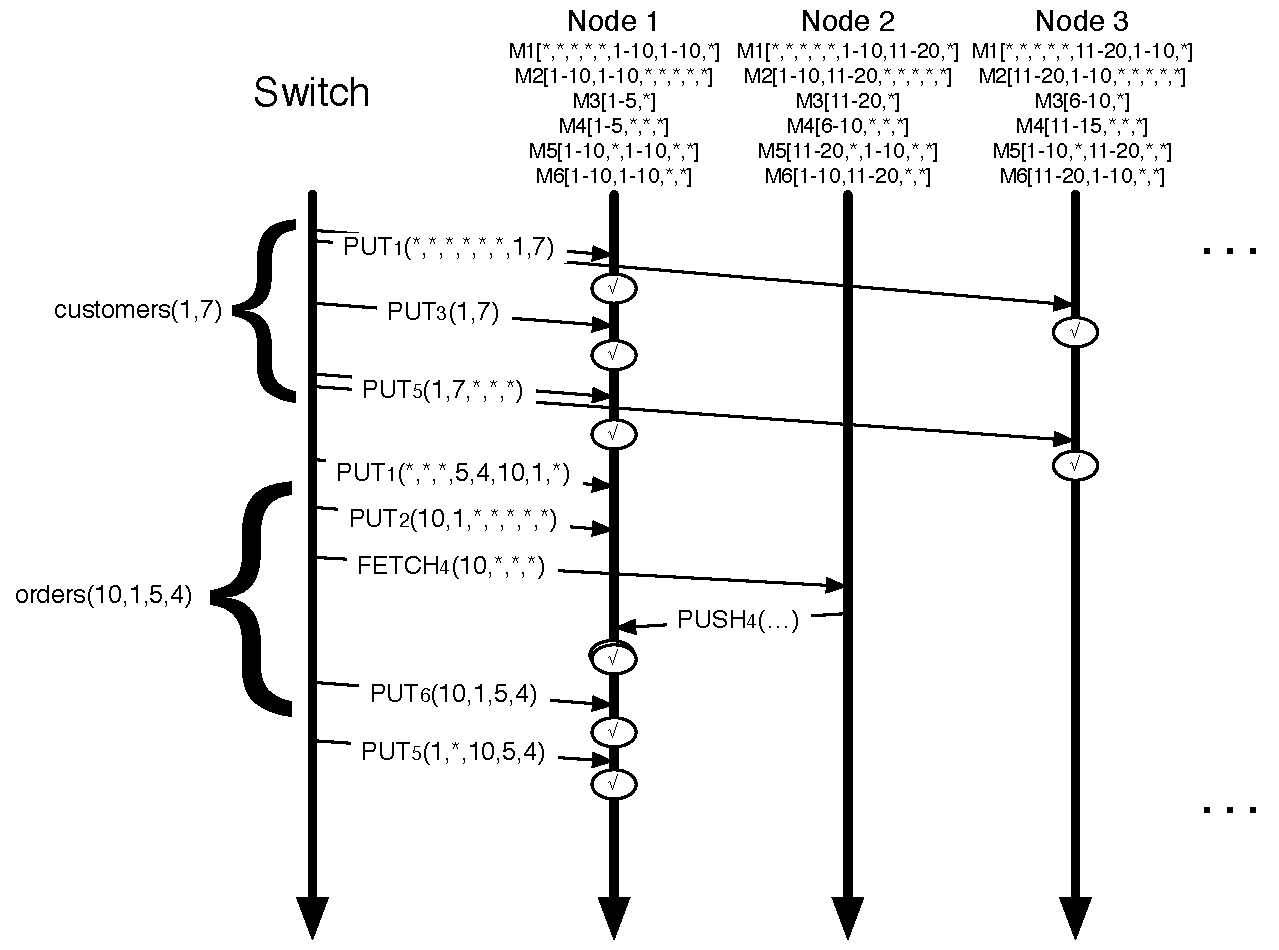
\includegraphics[width=3.5in]{images/MessageFlow.pdf}
\caption{Sequence diagram.}
\end{center}
\end{figure}



\begin{figure}
\begin{center}
\textbf{Schema}
\end{center}
\begin{algorithmic}
\STATE \textbf{create table} customers(cid \textit{int}, nation \textit{int}); 
\STATE \textbf{create table} orders(
\STATE \hspace*{0.1in} oid \textit{int}, o\_cid \textit{int}, opriority \textit{int}, spriority \textit{int},
\STATE \hspace*{0.1in}  \textbf{foreign key}(o\_cid) \textbf{references} customers(cid)
\STATE );
\STATE \textbf{create table} lineitems(
\STATE \hspace*{0.1in} l\_oid \textit{int}, lateship \textit{int}, latedelivery \textit{bool}, shipmode \textit{bool},
\STATE \hspace*{0.1in} \textbf{foreign key}(l\_oid) \textbf{references} orders(oid)
\STATE );
\end{algorithmic}
\begin{center}
\textbf{Query}
\end{center}
\begin{algorithmic}
\STATE \textbf{select} count(*),
\STATE \hspace*{0.1in} nation, cid, oid, opriority, spriority, 
\STATE \hspace*{0.1in} lateship, latedelivery, shipmode 
\STATE \textbf{from} customers, orders, lineitems 
\STATE \textbf{where} o\_cid=cid and l\_oid=oid 
\STATE \textbf{group by cube} 
\STATE \hspace*{0.1in} nation, cid, oid, opriority, spriority, 
\STATE \hspace*{0.1in} lateship, latedelivery, shipmode;
\end{algorithmic}
\caption{An example query that constructs a warehouse for analyzing customer behavior with respect to shipping.  Given a table of customers, orders, and lineitems in those orders, the query builds a datacube over the full join of those tables.}
\label{fig:example}  
\end{figure}


\section{Algorithms from the Arhitecture Section}


\begin{figure}
\begin{algorithmic}[1]
\STATE $Msgs \leftarrow \emptyset$
\FORALL{Update $U \in$ Trigger}
	\STATE Region $Reg = \pi_{U.target.loop\_vars} \left(index(U.target\_map)\right)$
	\FORALL{Partition $\{P | P\in U.target\_map \wedge (P \cap Reg \neq \emptyset)\}$}
		\STATE $Reads = \emptyset$
		\FORALL{Ref $R \in get\_map\_refs(U.expression)$}
			\STATE $RReg \leftarrow \pi_{R.loop\_vars} P$
			\STATE $RPart \leftarrow \{RP | RP\in R.map \wedge (RP \cap RReg \neq \emptyset)\}$
			\STATE $Reads \leftarrow Reads \cup \{(ReadP.node, R)\}$
		\ENDFOR
		\STATE $Reads \leftarrow group\_by\_node(Reads)$
		\STATE $Msgs \leftarrow put(U, P, Reads.size)$
		\FORALL{$($Node $N, \{$Ref $R\}) \in Reads$}
		  \STATE // PUSH results to $P.node$
			\STATE $Msgs \leftarrow fetch(N, \{R\}, P.node)$
		\ENDFOR
	\ENDFOR
\ENDFOR
\end{algorithmic}
\caption{The Switch's trigger dispatch algorithm}
\label{alg:dispatch}
\end{figure}


\begin{figure}
\begin{algorithmic}[1]
\STATE Given: Update $U$
\FORALL{Ref $R \in U.expression$}
	\STATE $Inputs \leftarrow Inputs \cup (R, \emptyset)$
\ENDFOR
\FORALL{$($Ref $InR,$ Value $V) \in \cup(msg_{PUSH})$}
	\FORALL{$(R, Table) \in Inputs$}
		\IF{$check\_match(InR, R)$}
			\STATE $Table \leftarrow Table \cup (InR.keys, V)$
		\ENDIF
	\ENDFOR
\ENDFOR
\FORALL{$(K,\{V\}) \in $ JOIN $ (Keys, Val) \in Inputs$}
	\STATE $Target = bind\_vars(U.target \leftarrow Keys)$
	\STATE $apply(Target, bind\_vars(U.expression \leftarrow \{V\}))$
\ENDFOR
\end{algorithmic}
\caption{The DW Node's collation algorithm}
\label{alg:collation}
\end{figure}


\section{Distributing the Switch}
\label{sec:distswitch}


The role of the switch is to provide a synchronization mechanism for the updates.  Specifically, the delta encoding approach used by the update rules requires that all update rules be applied to a consistent snapshot of the maps.  The current implementation of Cumulus performs this synchronization at a single node.  However, limiting the switch to only one node creates a scaling bottleneck.  

Despite the cloud computing mantra of rejecting consistency, this application requires it.  Complex locking protocols have poor scaling performance, so a simpler, lock-free protocol is required.  We achieve this goal by introducing the notion of \textit{pipeline scheduling}.  Pipeline scheduling exploits the acyclicity of compiler-generated data-flow graphs to allow nodes to correctly interleave and process update rules with only limited network overhead and processing latency.


{\em Pipeline Scheduling}.
Loose clock synchronization between nodes is assumed, and allows time to be partitioned into a sequence of numbered ticks, each lasting on the order of seconds.  When a set of updates is triggered, a switch node sends tentative put requests to all participating nodes.  These nodes respond with their current tick counter, and the switch forwards the maximum returned tick to all nodes.

The updates are considered to have been posted at the maximum returned tick.  However processing is deferred for a number of ticks equal to the depth of the map being updated.  The result is a data-flow process resembling a parallelized CPU pipeline.

During a given tick, all updates scheduled for processing are evaluated.  Once all updates scheduled for the tick have completed, the node responds to FETCH requests for the tick with PUSH messages.  Recall that each edge in the data flow graph represents a FETCH request for a specific update.  The difference in depth between the edge's ends is the number of ticks in advance of the PUT that the response is sent.  

For example, in Figure \ref{fig:dataflow} without removing any edges,
$Depth(q) = 2$, $Depth(qC) = 1$, and $Depth(qO2) = 0$.  Updates to map $q$ scheduled for processing during tick 4 would receive data from map $q_C$ during tick 3, and from map $q$ during tick 2.


\subsection{Old Consistency Stuff}


For consistency, an update's effect on the warehouse be logically atomic.  Atomicity is of particular importance, since the set of update rules triggered by a given update switch typically span the breadth of the data-dependency graph; Updates to any input relation typically have at least one read to a map updated by every other relation.

As the clearinghouse for updates, the Switch presents an ideal point for generating a total ordering over all tuples to be inserted into the warehouse.  The Switch maintains a version number for each node, incremented on every PUT dispatched to the node hosting it.  FETCHes sent to that node are tagged with the version number of the last PUT sent to the node, while PUTs are dependent on the completion of the prior PUT.

DW nodes ensure consistent evaluation of updates by buffering PUT requests received out of order, or prior to the completion of an earlier PUT request.  Similarly, FETCH requests for a particular version are buffered until the corresponding PUT request has completed, if it has not already done so.

Periodically, the switch queries each node for the completion status of pending PUT requests.  For each node, it computes the lowest FETCH version number for a read associated with an incomplete PUT request.  The Switch then disseminates these version numbers throughout the warehouse with a COMMIT message.  When a node receives a COMMIT, it snapshots its maps by discarding all updates for values that were overwritten before the commit version.


\subsection{Precomputing message groups in the switch}

{\em Indexing message sets}.
To streamline the dispatch of messages to component nodes, the switch pre-generates a spatial index for each template\footnote{Elsewhere called map update statement. It is convenient to think of such a statement, particularly if it is of the {\tt foreach} form, as a template of message passing.}, similar to the grid file directory.  Every entry in the spatial index contains a set of PUT and FETCH messages.  When the template is triggered, the tuple's values are used to index into the spatial index and the corresponding messages are parametrized and sent.  The algorithm for generating the spatial index is presented in Figure \ref{alg:dispatch}.




\section{Related Work}
\label{sec:relatedwork}


Database compilers \cite{DBLP:conf/pods/Batory88,DBLP:journals/jiis/BatoryT97}.

A large body of previous research has focused on incremental view maintenance
of relational database queries
\cite{roussopoulos-tods:91,griffin-sigmod:95,colby-sigmod:96,yan-vldb:95,kotidis-tods:01,zhou-vldb:07}.
The focus of this work was always on only one level of delta rewriting
and then using classical relational query processing techniques
based on interpreted query plans and heavyweight monolithic query operators
(such as joins).
In general, however, this means
that the rewritten query is still an arbitrarily complex query (in the number
of joins) and the message passing technique employed in Cumulus is not
applicable.

Most of the previous work on incremental view maintenance does not observe or leverage the fact that aggregation in queries can actually make incremental maintenance {\em easier}, rather than harder, because it greatly reduces the amount of data in the result and because numbers have additional algebraic properties that relations do not have and which allow for further decomposition and optimization of queries.

Column stores \cite{DBLP:journals/tods/Batory79,DBLP:conf/cidr/KerstenM05,DBLP:conf/vldb/StonebrakerMAHHH07}
are a prominent and successful instance of the recent trend
to abandon rather old database technologies and try out new architectural
para\-digms. Column stores have also been shown to be particularly well suited
for OLAP. However, column stores are fundamentally a secondary storage
concept; in main memory, it does not seem to be particularly meaningful to talk of column or row stores. To date, there has also been no work
on incremental view maintenance in column stores.
Indeed, they are notoriously bad at updating (worse than classical row stores).

H-Store is an OLTP system that abandons classical concurrency control and
recovery baggage for very high performance. It is interesting for the
fresh look at things, and for the viewpoint that even OLTP systems should
be much simpler, nimbler systems than classical databases, which is also
part of the vision behind Cumulus. However, H-Store solves a problem very
different from the one addressed by Cumulus.

Recently, a number of startups have taken off with the idea of running
databases -- even classical technology such as Postgres -- in the cloud
(e.g. Greenplum and Aster Data). While several systems aim at OLAP
applications, none of them allows for true online aggregation as Cumulus does,
and none of the systems takes as radical a lightweight, systemsy approach
as Cumulus.
